\section{Introduction}
We consider the following problem of generating patterns by drawing rectangles.
A target pattern is given as a grid of black and white cells.
We begin with a white grid and place solid black or white rectangles, each rectangle covering any previously placed rectangles.
Placing arbitrary sized rectangles makes the problem NP-hard, so we consider only placing rectangles that extend either the full height or width of the grid.
Our goal is to find the smallest number of rectangles required to create the target pattern.
\label{s_intro}

\subsection{Problem Definition}

Define a pattern $P$ to be an $n_{R} $ by $n_{C}$ grid of black and white squares. Let $n = n_R + n_C$.
%See Fig.~\ref{fig:example_pattern} for an example of a pattern.

%\begin{figure}[h]
%\centering
%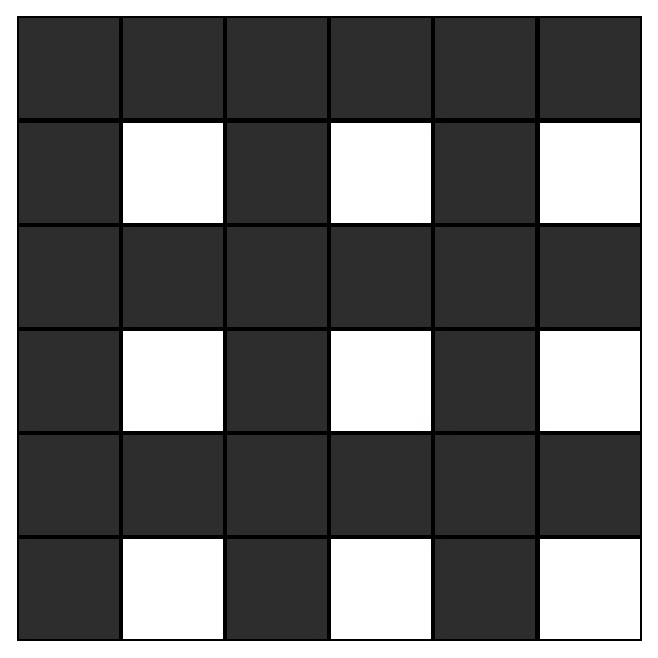
\includegraphics[width=3cm]{example_pattern}
%\caption{An example of a black and white pattern}
%\label{fig:example_pattern}
%\end{figure}

A rectangle strip-rule on $P$ is either a black or white rectangle that extends from one side of the pattern to the opposite side.
Precisely a rectangle in $P$ is either a set of contiguous rows of $P$ or a set of contiguous columns of $P$

A rectangle strip-rule list (a SRRL) that generates $P$ is an ordered list of rectangle strip-rules, that when applied in ordered to a blank (white) grid the size of $P$ create the target pattern. See Fig.~\ref{fig:pattern_generation} for an example of a pattern generated by a SRRL.

\begin{figure}[h]
\centering
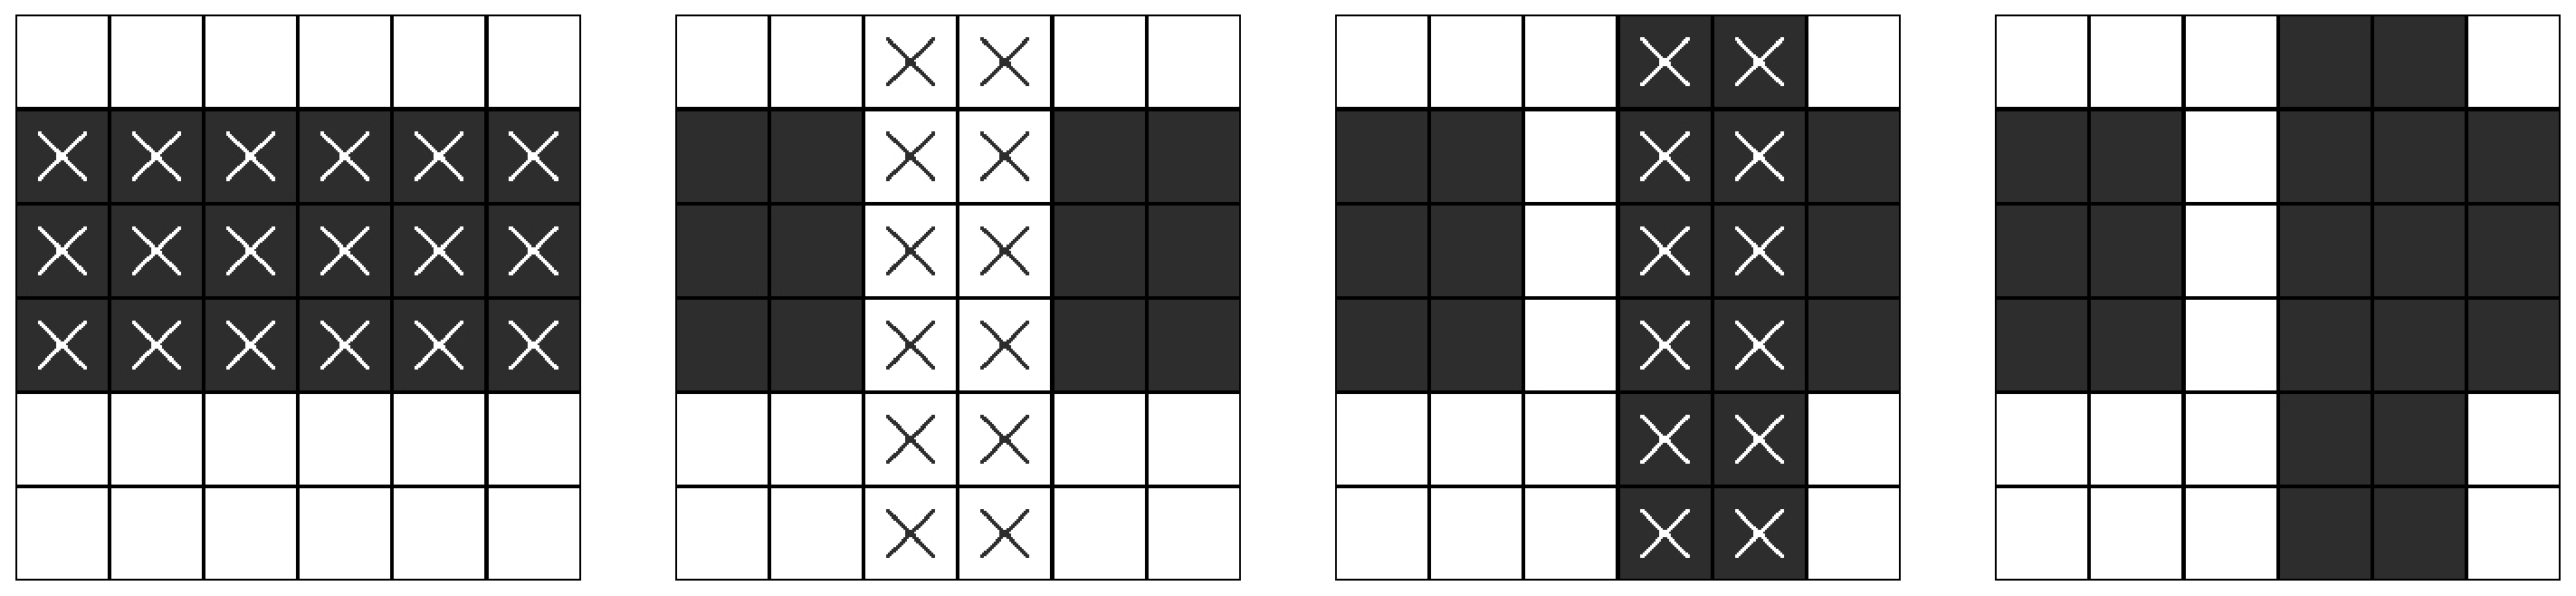
\includegraphics[height=3cm]{pattern_generation}
\caption{A pattern generated by a SRRL of 3 elements}
\label{fig:pattern_generation}
\end{figure}

We say a pattern $P$ is a strip-rule pattern if there is a SRRL that generates $P$. Note that not every pattern $P$ is a strip-rule pattern. See Fig.~\ref{fig:checkerboard} for an example of a pattern that is not a strip-rule pattern.

\begin{figure}[h]
\centering

\includegraphics[width=1.5cm]{checkerboard}
\caption{The $2 \times 2$ checkerboard: an example of a pattern that is not a strip-rule pattern}
\label{fig:checkerboard}
\end{figure}

% Our goal on this paper is, given a pattern $P$ of dimensions $n_{R} \times n_{C}$, finding if $P$ is a strip-rule pattern and, if so, finding a minimal SRRL for it.

An SRRL is considered optimal if it has the minimum number of rectangle strip-rules of any SRRL that generates $P$.


\subsection{Problem Background}

\subsubsection{Rectilinear Pictures and Access Control Lists.}
The method of stacking rectangles to create patterns has applications in both graphics and network routers.
A common method for drawing graphics is to allow the user to repeatedly apply a rectangle tool to a blank canvas (See Xfig or PowerPoint).
Each rectangle is of a solid color and covers everything in a defined rectangular region.
This sequence of rectangles drawn can be represented by a rectangle rule list (RRL).
The problem of finding the minimum length RRL needed to create a given pattern is a generalization of the SRRL problem we explore.

Alternatively, instead of being given an $n_{R} $ by $n_{C}$ grid as input,
one can start with the numbers $n_{R}$ and $n_{C}$, and a list of $m$ rules.
The goal is to find a minimum-length list that gives the same pattern as the
input list. As shown in an extended version of \cite{ACJKLW07},
it is possible to
construct the $n_{R} $ by $n_{C}$ grid in time $O(n_R \cdot n_C + m^2)$.

One important application of RRLs is in access routers.
An Internet Service Provider might use access control lists (ACLs) on network router line cards in order to choose whether to forward or drop a packet based on the sending or receiving IP address.
This decision could be answered by checking a two-dimensional Boolean array based on the sender and receiver IP addresses.
This problem can be translated into a restricted version of our RRL problem.
An in depth discussion of this translation and its properties is discussed in detail in "Applegate et al."'s paper \cite{ACJKLW07}.
In ACLs minimization, the rectangles are of the certain form:
$n_R$ and $n_C$ are powers of two, rows and columns are
indexed with binary strings
from $0^w$ to $1^w$,  and each rectangle must be given by
two prefixes $y$ and $z$ of length at most $w$ each;
the actual rectangle consists of the rows whose index has
 $y$ as a prefix and the columns who have $z$ as prefix.



\subsubsection{Related Work.}
Unfortunately, the general problem of finding minimum length RRLs has been shown to be NP-Hard by \cite{ACJKLW07}.
Instead, we work on a restricted version of the problem in which any rectangle rules applied must extend either the height or width of the original pattern and only black or white rectangles are allowed.
This 2-color strip-rule problem was originally posed in "Applegate et al."'s paper
\cite{ACJKLW07}, where an optimal solution is given in $O(n^3)$-time, where $n$ is the sum of the height and width of the original pattern.
\cite{ACJKLW07} obtains an optimal solution to the strip-rule version of the
ACL problem with a similar (but more complicated) $O(w n^3)$-time algorithm.
A 1.5 ratio approximation algorithm is given for the problem in $O(n^2)$-time.
While there exist numerous results related to various other restricted problems regarding RRLs, we know of no other work related to this 2-color strip-rule problem.

ACL can be used in firewalls \cite{KRRW12}.
\cite{KRRW12b} introduce axioms with the goal of
creating and analyzing algorithms for optimizing the rewriting of rules
in Software Defined Networks.
\cite{LMT10} consider classifiers in dimensions higher than two,
which reduce to either ACL or RRL lists in dimension two. They propose
and experimentally evaluate heuristics without performance guarantees,
as well as relate these classifiers to the Firewall Decision Diagrams of
\cite{GL07}.
\cite{PL14}, and \cite{CDG16}  also consider higher dimensional classification based on rules.
\cite{KLRW13} and \cite{ZNHBM14} introduce more general rule-minimization problems.
\cite{SK10} uses rule minimization as a start for solution to an
extended problem. Efficiently
removing redundant rules has been proposed in \cite{SK10b}.

The complexity of finding minimum length ACLs in two dimensions
is still unknown, but with an arbitrary
number of dimensions, this problem is NP-hard \cite{KNCER13}.
\cite{ACJKLW07} gives a $O(\min(m^{1/3},\OPT^{1/2}))$-approximation
algorithm for finding minimum length RRLs, where $m$ is the length
of the input $RRL$. This is still the best published ratio.

\cite{DLT16} provides heuristics for higher-dimensional ACL and RRL
minimization
(\cite{DLT16} calls the ACLs minimization prefix-ACL, while
range-ACL is their terminology for finding minimum length RRLs),
on the way improving the approximation ratios provided by
 \cite{ACJKLW07} for ACLs minimization.  The approximation
algorithms of \cite{DLT16}  and \cite{ACJKLW07} use
as a subroutine the strip-rule version that we study.


\subsubsection{Our Results.}
Using the structure defined in "Applegate et al."'s \cite{ACJKLW07}
$O(n^3)$ exact algorithm for 2-color SRRLs,
we give an improved $O(n^2 $ log $n)$ exact algorithm for the SRRL problem.
Given the similar structures of the RRL and ACL optimal solutions given by
\cite{ACJKLW07}, we expect our solution can be extended to improve the
running time of an exact algorithm
for the strip-rule ACL problem from $O(wn^3)$ to  $O(w n^2$ log $n)$.
As strip-rule ACLs occur in high percentage
of ACL minimization cases \cite{ACJKLW07}, this is one reason to study SRRL.
Another two reasons are: we believe SRRL is a natural problem, and  SRRL is used in the approximation algorithms for RRL minimization.

Our result is obtained by digging deeper in the structure of the
dynamic programming of \cite{ACJKLW07} combined with use of
geometric data structures to speed up the process.
We use fast two-dimensional orthogonal range queries,
using existing data structures  (a time bound of $O(\log n)$ time
 per query being textbook material \cite{KOS2000}).



\subsection{Organization}
We begin by defining all structures and concepts relevant to finding the optimal SRRL.
Next we give a detailed explanation of our $O(n^2$ log $n)$ optimal algorithm.
Finally, we state all theorems that make the algorithm possible and analyze the algorithm's time and space complexity.
